\documentclass[letterpaper,10pt,onecolumn]{IEEEconf}
% \documentclass[letterpaper,10pt,draftclsnofoot,onecolumn]{IEEEconf}

\usepackage{amsmath,amssymb}
\usepackage{graphicx,color,xspace}
\usepackage[ruled, vlined]{algorithm2e}

\newcommand{\reals}{\mathbb{R}}
\DeclareMathOperator*{\argmin}{argmin}

\begin{document}

\title{Homework 3 - Coordinate Descent}
\author{Evan Gravelle \quad \quad November 21, 2016}
\maketitle

\section{Method}

Coordinate descent is method for solving an optimization problem by optimizing over one coordinate at a time. The objective in this homework was to minimize $L(w)$ where $w \in \reals^p$. Once a coordinate $j$ is selected, $w(t+1) = \argmin\{L(w-\overline{\alpha}), L(w), L(w+\overline{\alpha})\}$ where $\overline{\alpha}$ is a one-hot vector with $\overline{\alpha}_j = \alpha$ and $\alpha$ is an exponentially decaying step size. The coordinate with the largest previous decrease in loss is chosen at each iteration, with previous decreases initialized as large values, and a reset of these values occurs every $q$ iterations. This algorithm does not require knowledge or continuity of the gradient of the loss.

\section{Convergence}

This algorithm will converge to the optimal loss if the loss is a convex function and if the step size starts out large enough and asymptotically approaches zero.

\section{Experimental Results}

The experimental results show that the custom algorithm converges faster than random coordinate selection. Both converge to the same accuracy, but the custom algorithm converges with less noise.

\begin{figure}[h]
\begin{minipage}{.5\textwidth}
\centering
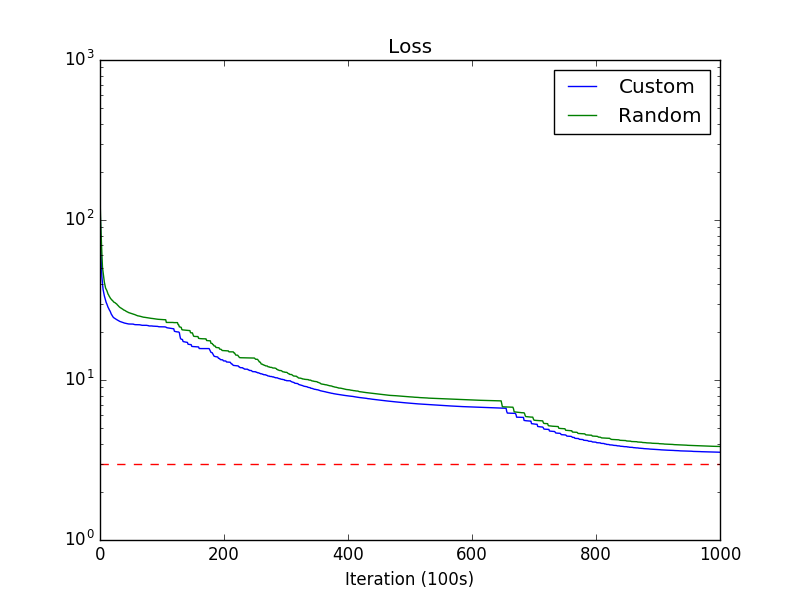
\includegraphics[width=\linewidth]{loss.png}
\end{minipage}
\begin{minipage}{.5\textwidth}
\centering
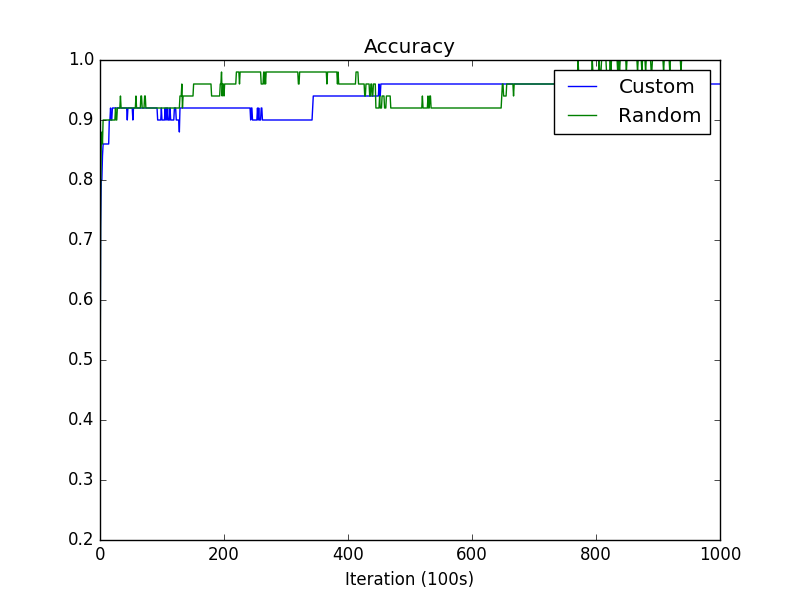
\includegraphics[width=\linewidth]{accuracy.png}
\end{minipage}
\end{figure}


\section{Critical Evaluation}

This coordinate descent algorithm could be improved in a few ways. If the gradient of the loss function is known, then the step size at each iteration can be calculated as a function of the gradient at the current point, to more accurately achieve a minimum with respect to a given coordinate. The prioritization of previous improvements with constant resets is quite heuristic, perhaps approximating how much the gradient has changed in each direction after each update would result in a smarter sequence of updates.

\end{document}